\documentclass[
    paper=a4, % Seitenformat
    fontsize=12pt,  % Schriftgröße
    oneside,        % einseitig
    headsepline,    % Trennlinie für die Kopfzeile
]{extarticle}         % KOMA-Script Article
%------------------------------------------------------------------------

\usepackage[automark]{scrlayer-scrpage}  % Seiten-Stil für scrartcl
\usepackage[utf8]{inputenc}              % Eingabekodierung
\usepackage[T1]{fontenc}                 % Zeichenkodierung
\usepackage[english,ngerman]{babel}      % Mehrsprachenumgebung, Hauptsprache Deutsch
\usepackage{setspace}
\usepackage{latexsym}                    % Latex-Symbole
\usepackage{amsfonts, amssymb, amstext}  % Mathematische Formeln
\usepackage{bbm}                         % bbm Schriftart
\usepackage{graphicx}                    % Abbildungen einbinden
\usepackage{tikz}                        % Abbildungen zeichnen
\usepackage{enumitem}
%\usepackage[outputdir=out]{minted}
\usepackage{mathtools}
\usepackage{pdfpages}
\usepackage[algo2e]{algorithm2e}
\usepackage{fontawesome}
\usepackage{hyperref}
\usepackage[backend=biber,style=numeric,url=true,sorting=none,doi=false,urldate=long,natbib=true]{biblatex}
\usepackage[a4paper,lmargin={3cm},rmargin={3cm},tmargin={2.5cm},bmargin = {2.5cm}]{geometry}
\usepackage{algorithm}
\usepackage{algpseudocode}
\usepackage{amsmath}
\usepackage{tabularx}
\usepackage{breqn}
\usepackage{neuralnetwork}
\usepackage{pgfplots}
\graphicspath{ {./images/} }

\pagestyle{scrheadings}                  % Kopfzeilen nach scr-Standard
\usetikzlibrary{automata}                % Tikz-Library zum Zeichnen von Automaten

\usepackage{csquotes}
\usepackage{amssymb}
\usepackage{subfiles}
\usepackage{authblk}
\MakeOuterQuote{"}

% Horizontale Linie mit Abstand zu den Seitenrändern
\newcommand{\ownline}{\vspace{.7em}\hrule\vspace{.7em}}
%\renewcommand{\ALG@name}{Algorithmus}
\newcommand{\RNum}[1]{\uppercase\expandafter{\romannumeral #1\relax}}
\newcommand{\qedwhite}{\hfill \ensuremath{\Box}}

\newtheorem{theorem}{Satz}[subsection]
\newtheorem{definition}[theorem]{Definition}
\newtheorem{example}[theorem]{Beispiel}
\newtheorem{bem}[theorem]{Bemerkung}
\newtheorem{satz}[theorem]{Satz}
\newtheorem{lemma}[theorem]{Lemma}

\addbibresource{Bachelorarbeit.bib}
% Biblatex Konfiguration
\DeclareFieldFormat{urldate}{\mkbibbrackets{#1}}
\DeclareNameAlias{sortname}{last-first}
%\DeclareFieldFormat{date}{(#1)}
\renewcommand*{\labelnamepunct}{\addcolon\addspace}
\renewcommand{\arraystretch}{1.7}
\numberwithin{equation}{section}

%-----------------------------------------------------------------------------------
%%% DOCUMENT-HEAD %%%
%-----------------------------------------------------------------------------------

% This info will be visible in the document head
%\author{Alexandro Jedaidi}
%\date{}

\linespread{1.25}
\begin{document}
    \begin{titlepage}
    \begin{center}
        \vspace*{1cm}
        %        \affil{
        %            \centering \\ \vspace{1cm}
        %            \small\scshape Universität Augsburg \\
        %            \small\scshape Mathematisch-Naturwissenschaftlich-Technische Fakultät
        %        }
        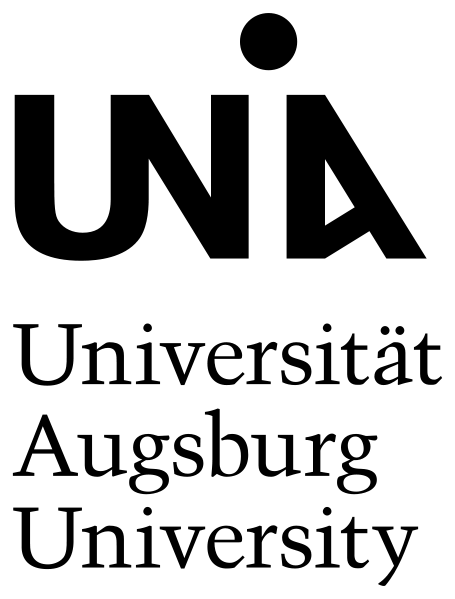
\includegraphics[width=4cm]{uni_aux_logo}
        \vspace{2.5cm}

        \Large
        \textbf{Vergleich der Integrationsmethoden und der Methoden des maschinellen Lernens für gewöhnliche
        Differentialgleichungen}

        \vspace{1.5cm}
        \textbf{Alexandro Jedaidi}\\
        Universität Augsburg \\
        Mathematisch-Naturwissenschaftlich-Technische Fakultät\\
        \today
    \end{center}
\end{titlepage}
    \newpage
    \tableofcontents
    \newpage
    \pagestyle{headings}

    \subfile{sections/einleitung.tex}

    \subfile{sections/problemstellung.tex}

    \subfile{sections/numerik.tex}

    \subfile{sections/MachineLearning.tex}

    \subfile{sections/anwendungsbeispiele.tex}

    \subfile{sections/resultat.tex}

    \newpage
    \printbibliography[heading=bibintoc]
    \newpage
    \phantomsection
    \addcontentsline{toc}{section}{\listfigurename}
    \listoffigures
\end{document}